\pdfoutput=1
\documentclass[11pt]{article}

\usepackage[margin=1in]{geometry}
\usepackage{amsmath}
\usepackage{amssymb}
\usepackage{array}
\usepackage{booktabs}
\usepackage{caption}
\usepackage{graphicx}
\usepackage{microtype}
\usepackage{placeins}
\usepackage{hyperref}
\usepackage[numbers,sort&compress]{natbib}
\usepackage{siunitx}
\usepackage{subcaption}
\usepackage{tikz}
\usepackage{xcolor}
\usepackage{xspace}
\usetikzlibrary{arrows.meta,positioning}

\hypersetup{
  colorlinks=true,
  linkcolor=blue,
  citecolor=blue,
  urlcolor=blue
}

\newcommand{\angstrom}{\text{\normalfont\AA}\xspace}
\newcommand{\calpha}{C\ensuremath{\alpha}\xspace}
\newcommand{\zB}{z_{\mathrm{B}}}

\title{Evaluating Persistent Sheaf Laplacian Descriptors for Protein Flexibility Prediction}
\author{Ryan Charette}
\date{}

\begin{document}
\maketitle

\begin{abstract}
Residue-level protein flexibility is central to catalysis, ligand recognition, allostery, and protein engineering, yet it remains difficult to infer from a single static structure. Crystallographic B-factors provide a widely available experimental proxy for atomic displacement, but their use in machine learning requires careful normalization and biological validation. Here, center-labeled persistent sheaf Laplacian (PSL) descriptors are used to encode multiscale local \calpha geometry, and Random Forest models are evaluated by five-fold cross-validation. Across 364 proteins and 78,419 residues, the primary center-labeled PSL model achieved a mean per-protein Pearson correlation coefficient (PCC) of 0.602 (95\% CI [0.588, 0.616]), pooled PCC of 0.571, and mean RMSE of 0.845 on within-protein normalized B-factors. A PSL+SHAP explanation model showed moderate alignment between residue attribution strength and normalized B-factor (absolute-attribution PCC 0.482, 95\% CI [0.465, 0.497]; top-quintile Jaccard overlap 0.338, 95\% CI [0.326, 0.350]). Biological validation on 348 annotated proteins and 75,215 residues showed that normalized B-factors increase with solvent-accessible area (mean Spearman $\rho=0.433$, 95\% CI [0.416, 0.449]) and decrease with local packing density ($\rho=-0.411$ for the largest packing scale, 95\% CI [-0.426, -0.396]). Flexible top-quintile residues were enriched among solvent-exposed residues (odds ratio 4.66, 95\% CI [4.23, 5.19]), under-packed residues (odds ratio 6.20, 95\% CI [5.59, 6.89]), and terminal residues (odds ratio 4.67, 95\% CI [3.07, 6.74]). Baseline comparisons on the common 274-protein subset showed that PSL descriptors improved on classical structural annotations alone (mean PCC 0.608 versus 0.575), while a simple \calpha graph baseline and a combined classical+PSL model achieved mean PCCs of 0.629 and 0.627, respectively. Protocol-comparability analyses gave much higher pooled PCCs under random residue-level raw-B-factor splits (0.853--0.898) than under protein-level raw-B-factor evaluation (mean per-protein PCC 0.600--0.605), although the same random-residue predictions averaged only 0.606--0.636 when summarized by protein. Split-dependence controls showed that classical structural and simple graph features also reached pooled random-residue PCCs near 0.85. These results support a moderate, biologically grounded predictive signal  from PSL features while showing that simple graph and combined geometric descriptors remain competitive.
\end{abstract}

\section*{Significance Statement}
Machine-learning models of protein flexibility are useful only when their predictions generalize across proteins and their explanations can be tied to independent structural biology. This study combines grouped predictive modeling, a targeted reproduction of evaluation protocols reported by Hayes et al., SHAP attribution, and residue-level biological validation. The results show that persistent sheaf Laplacian descriptors capture a reproducible geometric signal associated with crystallographic flexibility, while also showing that high raw-B-factor scores under random residue-level splits should not be interpreted as protein-independent generalization.

\section{Introduction}
Protein function depends on conformational heterogeneity across multiple spatial and temporal scales. Catalytic loops reorganize during turnover, binding pockets adapt to ligands, and allosteric communication often emerges from distributed changes in mobility. Because many proteins have experimentally determined structures but limited dynamical measurements, a central computational question is whether residue-level flexibility can be inferred from structural information alone.

Crystallographic B-factors are a practical target for this problem. For atom $i$, the isotropic B-factor is related to mean-square displacement by
\begin{equation}
B_i = 8\pi^2 \langle u_i^2 \rangle .
\end{equation}
B-factors are not pure dynamical observables: they are influenced by refinement protocols, crystal contacts, occupancy, resolution, and static disorder. Nevertheless, they remain one of the largest residue-level experimental signals linked to local mobility. A robust flexibility model should therefore generalize across proteins and should connect its learned signal to independent structural features known to influence mobility.

Structure-only prediction is challenging because local mobility depends on both immediate contacts and broader geometric context. Surface exposure, weak packing, termini, and flexible secondary-structure environments can all elevate B-factors, but these effects interact with global fold topology and local steric constraints. This motivates representations that encode not only local density, but also multiscale neighborhood organization.

Persistent sheaf Laplacians provide a spectral description of multiscale local geometry. In contrast to scalar graph descriptors, sheaf-based constructions can encode how local assignments vary across simplicial structure, producing eigenvalue summaries that reflect local connectivity and geometric organization. These descriptors are well matched to protein flexibility because residue motion is shaped by the surrounding structural neighborhood rather than by residue identity alone.

A second challenge is methodological. Reported B-factor prediction performance can change substantially depending on whether residues from the same protein are split across training and test sets, whether raw or within-protein normalized B-factors are used, and whether metrics are pooled across residues or averaged within proteins. For models intended to generalize to unseen structures, protein-level evaluation is therefore essential.

This study evaluates PSL descriptors for residue-level B-factor prediction. The contributions are fivefold: (i) prediction of within-protein normalized B-factors from center-labeled PSL descriptors; (ii) reproduction and comparison of selected Hayes et al. evaluation protocols to separate raw-B-factor approximation from protein-level generalization; (iii) baseline comparisons against classical structural annotations and simple \calpha graph descriptors; (iv) SHAP attribution analysis for PSL features; and (v) biological validation against solvent exposure, packing density, terminal position, and secondary-structure code.

\section{Background and Related Work}
\subsection{B-Factor Prediction and Elastic Network Models}
Classical approaches to protein flexibility often model structures as elastic networks. Gaussian network models (GNM) and anisotropic network models (ANM) represent residues as nodes connected by springs, using normal-mode behavior to estimate collective fluctuations \citep{haliloglu1997, atilgan2001, bahar2010}. These models are attractive because they are physically motivated and require few parameters, but their accuracy can depend on cutoff choices, coarse-graining, and the extent to which crystallographic B-factors reflect intrinsic motion rather than experimental context.

Flexibility-rigidity index (FRI) methods provide another influential family of geometric predictors. FRI encodes residue flexibility through kernel-weighted neighborhood rigidity and has shown strong performance for B-factor prediction across benchmark sets \citep{nguyen2016}. These methods reinforce a central biophysical premise of the present work: residue mobility is strongly tied to local packing and multiscale geometry.

\subsection{Topological and Sheaf-Based Descriptors}
Topological data analysis has been used to represent biomolecular structure through persistent homology, multiscale simplicial complexes, and spectral summaries \citep{edelsbrunner2010, xia2014}. Persistent sheaf Laplacians extend this idea by combining sheaf-theoretic assignments with persistent spectral information. For proteins, such descriptors can summarize local geometric organization across filtration scales, potentially capturing neighborhood constraints not available from pairwise contact counts alone. Hayes et al.~\citep{hayes2025, hayes2025correction} recently applied PSL descriptors to protein B-factor prediction and reported strong performance under several evaluation settings. The present work reproduces selected feature, target, and split choices from that prior study for comparison, while evaluating how metric aggregation and protein-level validation affect the interpretation of performance.

\subsection{Explainable Machine Learning in Structural Biology}
Explainable machine learning tools can help identify which features drive a model prediction, but explanation quality depends on the evaluation design. SHAP values provide an additive feature-attribution framework grounded in Shapley values \citep{lundberg2017}. In structural biology applications, SHAP should be interpreted as a model diagnostic rather than a causal assay: attributions indicate how a fitted model uses features, not whether those features independently cause flexibility. The present analysis evaluates SHAP attribution-target agreement for model predictions.

\section{Methods}
\begin{figure}[htbp]
\centering
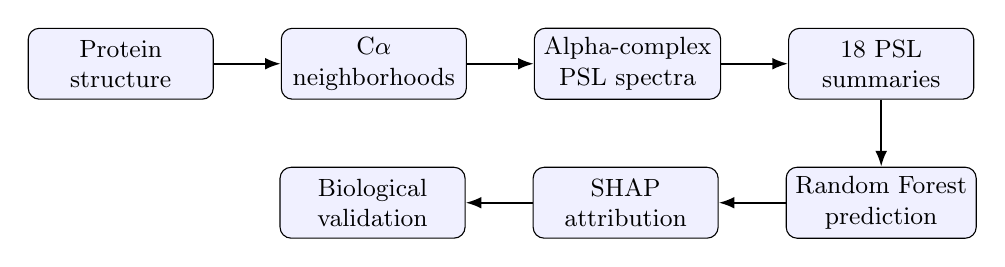
\begin{tikzpicture}[
  node distance=0.85cm,
  workflowstep/.style={draw, rounded corners, align=center, fill=blue!6,
    minimum width=2.35cm, minimum height=0.9cm, font=\small},
  arrow/.style={-{Latex[length=2mm]}, thick}
]
\node[workflowstep] (structure) {Protein\\structure};
\node[workflowstep, right=of structure] (neighborhoods) {\calpha\\neighborhoods};
\node[workflowstep, right=of neighborhoods] (spectra) {Alpha-complex\\PSL spectra};
\node[workflowstep, right=of spectra] (features) {18 PSL\\summaries};
\node[workflowstep, below=of features] (model) {Random Forest\\prediction};
\node[workflowstep, left=of model] (shap) {SHAP\\attribution};
\node[workflowstep, left=of shap] (validation) {Biological\\validation};
\draw[arrow] (structure) -- (neighborhoods);
\draw[arrow] (neighborhoods) -- (spectra);
\draw[arrow] (spectra) -- (features);
\draw[arrow] (features) -- (model);
\draw[arrow] (model) -- (shap);
\draw[arrow] (shap) -- (validation);
\end{tikzpicture}
\caption{Workflow for PSL flexibility prediction and explanation.}
\label{fig:workflow}
\end{figure}

\subsection{Data and Preprocessing}
Protein structures, residue-level B-factors, and annotation tables were taken from the MDG\_bfactor dataset \citep{feng2025}. PSL feature generation used the 365-protein structural collection, yielding usable PSL matrices for 364 proteins and 78,419 \calpha residues. Biological validation used the supplied \texttt{features-blind-prediction} annotation tables, yielding 348 proteins and 75,215 \calpha residues after matching available labels and annotations. Raw third-party structures and annotation tables were not redistributed with the analysis repository.

\begin{table}[htbp]
\centering
\caption{Dataset summary.}
\label{tab:dataset_summary}
\resizebox{\textwidth}{!}{%
\begin{tabular}{lrrrr}
\toprule
Dataset & Proteins & Residues & Mean residues/protein & Notes \\
\midrule
PSL feature set & 364 & 78,419 & 215.4 & Primary predictive analysis \\
Biological annotation set & 348 & 75,215 & 216.1 & Validation annotations available \\
Baseline comparison subset & 274 & 62,065 & 226.5 & Annotation, PDB, and PSL rows aligned \\
Small stratum & 30 & 907 & 30.2 & PSL predictive subset \\
Medium stratum & 36 & 3,246 & 90.2 & PSL predictive subset \\
Large stratum & 34 & 5,404 & 158.9 & PSL predictive subset \\
365-only stratum & 264 & 68,862 & 260.8 & Remaining PSL proteins \\
\bottomrule
\end{tabular}%
}
\end{table}

\subsection{Computational Reproducibility}
All predictive analyses were implemented as command-line Python scripts, and all reported uncertainty intervals use fixed random seeds documented in the repository configuration files. Lightweight metric snapshots are stored with the repository, while full prediction tables and PSL feature matrices are treated as derived artifacts that can be regenerated from the documented commands. Because the upstream research implementation used to compute persistent sheaf Laplacians did not expose an explicit redistribution license at package preparation time, the public repository uses a loader for a locally supplied copy of that implementation rather than redistributing the third-party source file.

\subsection{Target Definition and Within-Protein Normalization}
For protein $p$, raw \calpha B-factors $B_{ip}$ were converted to within-protein z-scores:
\begin{equation}
z_{\mathrm{B},ip} = \frac{B_{ip} - \mu_p(B)}{\sigma_p(B)}.
\end{equation}
This target focuses the learning problem on relative residue-level flexibility within each structure rather than absolute crystallographic scale differences across structures. For enrichment and overlap analyses, flexible residues were defined as the top 20\% of normalized B-factors within each protein. This percentile definition avoids imposing a universal raw B-factor threshold across structures with different resolution, refinement, and scale properties.

\subsection{Persistent Sheaf Laplacian Descriptor Construction}
Each protein was represented as a \calpha point cloud. For residue $i$ with \calpha coordinate $x_i$, local neighborhoods were defined by
\begin{equation}
X_i(r) = \{x_j : \lVert x_j - x_i \rVert_2 \le r\},
\quad r \in \{6, 9, 12\}\ \angstrom .
\end{equation}
For each neighborhood, an alpha complex was constructed using GUDHI. The primary descriptor used a center-labeled nonconstant sheaf: the target \calpha atom was assigned label 0 and all neighboring \calpha atoms were assigned label 1. The PSL degree was zero and the filtration width was $p=0$. In this setting, the degree-zero PSL summarizes how the distinguished center atom is embedded in the local alpha-complex neighborhood. Zero eigenvalues reflect local component structure, while nonzero eigenvalues summarize the strength and organization of local connectivity.

For each radius, the eigenvalue spectrum of the degree-zero PSL matrix was summarized by six statistics:
\begin{equation}
\max(\lambda_{\neq 0}),\quad \min(\lambda_{\neq 0}),\quad
\operatorname{mean}(\lambda_{\neq 0}),\quad
\operatorname{median}(\lambda_{\neq 0}),\quad
\operatorname{std}(\lambda_{\neq 0}),\quad
\#\{\lambda: |\lambda| \le 10^{-8}\}.
\end{equation}
If a neighborhood contained fewer than two \calpha atoms, the descriptor was set to zero-valued nonzero-eigenvalue summaries and the observed zero-eigenvalue count. The resulting feature vector contains 18 PSL descriptors per residue. Feature names encode radius, filtration width, degree, and statistic, for example \texttt{r12\_p0p0\_d0\_mean} denotes the mean nonzero eigenvalue at the 12~\angstrom neighborhood scale. Sensitivity analyses also evaluated the 15-feature median-only center-labeled descriptor, a 7/10/13~\angstrom standard-deviation descriptor, a constant-sheaf ablation, and a focused persistence-width and label-scaling sensitivity analysis.

\subsection{Predictive Models and Baselines}
The primary predictive model was a Random Forest regressor trained on residue-level PSL features. The main configuration used 2,000 trees, maximum depth 12, minimum samples per leaf 2, square-root feature sampling, and bootstrap sampling.

Baseline models were evaluated under the identical target definition, evaluation protocol, 1,000-tree Random Forest class, and uncertainty procedure on the common subset with aligned annotation, PDB, and PSL rows. The residue-position baseline used normalized residue index, terminal distance, terminal-decile indicator, sequence length, and inverse sequence length. The classical structural baseline used solvent-accessible area, three packing-density descriptors, position features, and one-hot secondary-structure source codes. The simple graph baseline used \calpha contact degrees and normalized degrees at 6, 8, 10, and 12~\angstrom, clustering coefficients at 8 and 12~\angstrom, and mean nearest-neighbor distances for 4, 8, and 12 neighbors. The combined model concatenated the classical structural descriptors and PSL descriptors.

\subsection{Model Evaluation}
Predictive models used 5-fold cross-validation grouped by protein, and target normalization was performed within each protein. Confidence intervals were computed by resampling proteins rather than residues.

\subsection{Protocol Comparability Analyses}
To separate representation quality from evaluation protocol, additional comparability analyses reproduced three PSL settings reported by Hayes et al.~\citep{hayes2025, hayes2025correction}. First, the PSL-only linear approximation corresponding to Hayes et al.'s Table~1 was audited using pooled and per-protein ordinary least squares, no/global/per-protein feature standardization, and optional per-protein affine rescaling of predictions, using 6/9/12~\angstrom median-summary PSL features and raw \calpha B-factors. Second, models following the blind-prediction setup in Hayes et al. used 7/10/13~\angstrom standard-deviation PSL features concatenated with the supplied annotation features, raw B-factors as the target, and 10-fold protein-level cross-validation with Random Forest and gradient-boosted decision-tree regressors. Third, the same raw-B-factor annotation+PSL feature set was evaluated under random \calpha-residue folds as a comparability check for atom-level splitting, with pooled, fold-mean, and protein-mean metrics reported separately. For the blind-prediction reproduction runs, PSL rows were aligned to annotation rows by exact row count when possible and otherwise by B-factor subsequence matching. This loaded 329 proteins and 72,069 residues: 273 exact row matches, 56 subsequence alignments, and 17 remaining alignment failures. These checks are intended to reproduce and diagnose the evaluation choices in one prior PSL study, not to treat those choices as community-wide benchmark standards.

As a split-dependence control, PSL-only, classical structural, simple graph, and classical+PSL feature sets were also evaluated on the exact-aligned 274-protein annotation subset using raw B-factors, 10-fold protein-level splits, 10-fold random residue-level splits, and the same 200-tree Random Forest configuration for all feature sets.

\subsection{SHAP Analysis}
The explanation model used 25 trees and maximum depth 8 to make SHAP computation tractable while preserving the predictive workflow. Residue-level attribution strength was defined as
\begin{equation}
I_i = \sum_m |\phi_{im}|,
\end{equation}
where $\phi_{im}$ is the SHAP value for feature $m$ at residue $i$. Explanation-target agreement was assessed by PCC and Spearman correlation between $I_i$ and the residue's normalized B-factor. Region-level agreement was assessed by the Jaccard index between top-quintile attribution residues $A$ and top-quintile B-factor residues $F$:
\begin{equation}
J(A,F) = \frac{|A \cap F|}{|A \cup F|}.
\end{equation}
Signed SHAP sums were reported separately because they track the model prediction relative to the SHAP baseline.

\subsection{Biological Validation}
Independent annotations were used to test whether the normalized B-factor labels follow expected structural biology. The main tests measured associations between normalized B-factor and solvent-accessible area, packing-density descriptors, terminal position, and secondary-structure code. Solvent exposure, weak packing, and chain termini are biologically meaningful sanity checks because they reflect reduced local constraints and increased opportunity for displacement. These annotations validate the coherence of the labels and learned signal; they do not establish that every high-B-factor residue is dynamically mobile in solution.

\subsection{Statistical Uncertainty}
For each protein, correlations, AUCs, standardized mean differences, and odds ratios were computed as appropriate. Confidence intervals and one-sided bootstrap p-values used protein-level resampling against explicit null values: 0 for correlations and standardized mean differences, 0.5 for AUC, and 1.0 for odds ratios. Bootstrap p-values are descriptive and were not adjusted for multiple testing. Predictive performance was summarized by per-protein PCC, per-protein Spearman correlation, per-protein RMSE, and pooled residue-level PCC.

\section{Results}
\subsection{PSL Descriptors Predict Normalized B-Factors}
Cross-validation showed a consistent moderate relationship between center-labeled PSL predictions and normalized B-factors. Across all 364 proteins, the mean per-protein PCC was 0.602 (95\% CI [0.588, 0.616]), the mean per-protein Spearman correlation was 0.574, the pooled residue-level PCC was 0.571, and mean RMSE was 0.845.

\begin{table}[htbp]
\centering
\caption{Predictive performance of PSL descriptors.}
\label{tab:predictive_performance}
\resizebox{\textwidth}{!}{%
\begin{tabular}{lrrrrrr}
\toprule
Dataset & Proteins & Residues & Mean PCC (95\% CI) & Mean Spearman & Pooled PCC & RMSE($\zB$) \\
\midrule
Small & 30 & 907 & 0.583 [0.491, 0.667] & 0.497 & 0.530 & 1.003 \\
Medium & 36 & 3,246 & 0.588 [0.534, 0.633] & 0.545 & 0.584 & 0.827 \\
Large & 34 & 5,404 & 0.573 [0.539, 0.604] & 0.579 & 0.566 & 0.828 \\
365-only & 264 & 68,862 & 0.610 [0.595, 0.624] & 0.586 & 0.575 & 0.832 \\
All & 364 & 78,419 & 0.602 [0.588, 0.616] & 0.574 & 0.571 & 0.845 \\
\bottomrule
\end{tabular}%
}
\end{table}

Performance was similar across size-defined subsets and the larger collection, indicating that PSL features carry residue-level signal across diverse protein length scales rather than being limited to a single dataset stratum.

\subsection{PSL Variant and Model Sensitivity}
PSL variants were evaluated to test whether center labeling, radius choice, spectral summary statistics, or gradient boosting materially changed performance. The center-labeled 6/9/12~\angstrom descriptor with both median and standard-deviation summaries gave the strongest center-labeled RF result, but the gain over the 15-feature center-labeled variants was small. A constant-sheaf ablation was statistically similar and slightly higher by mean PCC. Histogram gradient boosting did not improve over the regularized Random Forest for the labeled variants.

\begin{table}[htbp]
\centering
\caption{PSL descriptor and model sensitivity.}
\label{tab:model_sensitivity}
\resizebox{\textwidth}{!}{%
\begin{tabular}{llrrr}
\toprule
Descriptor & Model & Trees & Mean PCC (95\% CI) & Pooled PCC \\
\midrule
Center-labeled, 6/9/12, median & RF & 1,000 & 0.598 [0.584, 0.612] & 0.562 \\
Center-labeled, 7/10/13, std & RF & 1,000 & 0.597 [0.583, 0.611] & 0.569 \\
Center-labeled, 6/9/12, median+std & RF & 1,000 & 0.602 [0.588, 0.616] & 0.571 \\
Center-labeled, 6/9/12, median+std & RF & 2,000 & 0.602 [0.588, 0.616] & 0.571 \\
Center-labeled, 7/10/13, std & HGBT & -- & 0.593 & 0.565 \\
Center-labeled, 6/9/12, median+std & HGBT & -- & 0.598 & 0.568 \\
Constant sheaf, 6/9/12, median & RF & 1,000 & 0.604 [0.590, 0.618] & 0.581 \\
\bottomrule
\end{tabular}%
}
\end{table}

\subsection{Protocol Comparability with Evaluation Settings Reported by Hayes et al.}
Reproduction checks based on evaluation settings reported by Hayes et al. showed that the apparent accuracy of PSL-based B-factor models depends strongly on both the fitting protocol and the metric aggregation. In the PSL-only raw-B-factor linear-regression audit, pooled OLS over all residues gave mean per-protein PCC 0.520 without feature scaling and 0.555 with per-protein feature standardization. In contrast, fitting a separate linear model within each protein gave mean per-protein PCC 0.707. Thus, the closest reproduction of the Hayes et al. Table~1 analysis is the per-protein approximation protocol, not a single pooled linear model. Per-protein affine rescaling of pooled-OLS predictions increased pooled PCC to 0.858, but it did not close the per-protein profile-correlation gap (mean PCC 0.528), illustrating why pooled raw-B-factor metrics are not interchangeable with per-protein profile metrics.

Raw-B-factor models following the Hayes et al. blind-prediction setup with annotation+PSL features gave similar mean per-protein PCCs under protein-level
cross-validation (0.600--0.605). Under random \calpha-residue folds, pooled and fold-mean PCCs increased to 0.853 for GBDT and 0.898 for RF. However, when those same random-residue predictions were summarized within proteins, the mean PCCs were 0.606 and 0.636. The high atom-level scores are therefore reproducible, but they largely reflect the easier residue-level split and pooled raw-B-factor aggregation rather than protein-independent generalization.

\begin{table}[htbp]
\centering
\caption{Protocol-comparability analyses. Raw-B-factor protocols use the target scale used in the reproduced settings from Hayes et al.; the main analysis uses within-protein normalized B-factors. Dashes indicate metrics that are not defined for a non-folded in-sample approximation.}
\label{tab:protocol_comparison}
\resizebox{\textwidth}{!}{%
\begin{tabular}{lllrrr}
\toprule
Protocol & Feature set & Model and split & Mean protein PCC & Pooled PCC & Mean fold PCC \\
\midrule
PSL-only approximation & PSL 6/9/12 median & Per-protein OLS & 0.707 & 0.886 & -- \\
Blind-prediction reproduction & annotation+PSL 7/10/13 std & GBDT, protein folds & 0.605 & 0.108 & 0.396 \\
Blind-prediction reproduction & annotation+PSL 7/10/13 std & RF, protein folds & 0.600 & 0.163 & 0.442 \\
Atom-level comparability & annotation+PSL 7/10/13 std & GBDT, residue folds & 0.606 & 0.853 & 0.853 \\
Atom-level comparability & annotation+PSL 7/10/13 std & RF, residue folds & 0.636 & 0.898 & 0.898 \\
Main normalized-B analysis & PSL 6/9/12 median+std & RF, protein folds & 0.602 & 0.571 & -- \\
\bottomrule
\end{tabular}%
}
\end{table}

\begin{table}[htbp]
\centering
\caption{Audit of the PSL-only linear-regression protocol corresponding to
Hayes et al.'s Table~1 on 364 proteins and 78,419 residues.}
\label{tab:table1_lr_audit}
\resizebox{\textwidth}{!}{%
\begin{tabular}{lllrrr}
\toprule
Fit & Feature scaling & Prediction rescaling & Mean protein PCC & Pooled PCC & Mean RMSE \\
\midrule
Pooled OLS & none & none & 0.520 & 0.298 & 8.16 \\
Pooled OLS & global z-score & none & 0.520 & 0.298 & 8.16 \\
Pooled OLS & per-protein z-score & none & 0.555 & 0.280 & 7.35 \\
Pooled OLS & none & per-protein affine & 0.528 & 0.858 & 4.15 \\
Per-protein OLS & none & none & 0.707 & 0.886 & 3.49 \\
Per-protein OLS & per-protein z-score & none & 0.707 & 0.886 & 3.49 \\
\bottomrule
\end{tabular}%
}
\end{table}

A focused persistence-width sensitivity analysis for the PSL-only approximation was nearly flat: mean PCC was 0.7066, 0.7066, 0.7067, and 0.7068 for $p=0$, 0.25, 0.5, and 1.0, respectively. Enabling label scaling reduced the corresponding mean PCCs to 0.692 for $p=0$ and 0.691 for $p=0.5$. These checks do not support persistence width or label scaling as the source of a material reproduction gap.

The split-dependence control confirmed that high pooled random-residue accuracy is not specific to PSL. On the exact-aligned 274-protein subset, classical structural features, simple graph features, and the classical+PSL combination all reached pooled random-residue PCCs of 0.855--0.862, while their protein-level pooled PCCs remained 0.131--0.167. Mean per-protein PCC changed much less across split types. This pattern indicates that random residue-level evaluation allows models to exploit protein-specific scale and shared structure, whereas protein-level evaluation better measures transfer to unseen proteins.

\begin{table}[htbp]
\centering
\caption{Split-dependence control on raw B-factors using a common 200-tree Random Forest on the exact-aligned 274-protein subset.}
\label{tab:split_dependence}
\resizebox{\textwidth}{!}{%
\begin{tabular}{lrrr}
\toprule
Feature set and split & Mean protein PCC & Pooled PCC & Mean fold PCC \\
\midrule
PSL-only, protein split & 0.518 & 0.210 & 0.359 \\
PSL-only, residue split & 0.531 & 0.503 & 0.503 \\
Classical structural, protein split & 0.563 & 0.131 & 0.370 \\
Classical structural, residue split & 0.583 & 0.857 & 0.857 \\
Simple graph, protein split & 0.606 & 0.167 & 0.436 \\
Simple graph, residue split & 0.618 & 0.855 & 0.855 \\
Classical+PSL, protein split & 0.607 & 0.136 & 0.418 \\
Classical+PSL, residue split & 0.626 & 0.862 & 0.862 \\
\bottomrule
\end{tabular}%
}
\end{table}

\subsection{Baseline Comparisons}
Baseline comparisons determine whether PSL descriptors add information beyond simpler geometric and structural features. On the common 274-protein subset, PSL descriptors improved on the residue-position baseline and the classical structural baseline. The simple graph baseline was strongest by both mean and pooled PCC, with the combined classical+PSL model close behind. Thus, PSL descriptors provide useful geometric signal, but they are best interpreted as complementary to other local structural descriptors rather than as a uniformly dominant standalone representation.

\begin{table}[htbp]
\centering
\caption{Baseline comparison on the common 274-protein subset.}
\label{tab:baseline_comparison}
\begin{tabular}{lrrrr}
\toprule
Feature set & Mean PCC (95\% CI) & Mean Spearman & Pooled PCC & RMSE($\zB$) \\
\midrule
Residue position & 0.319 [0.294, 0.346] & 0.138 & 0.203 & 0.943 \\
Classical structural & 0.575 [0.558, 0.592] & 0.536 & 0.518 & 0.818 \\
Simple graph & 0.629 [0.614, 0.644] & 0.606 & 0.612 & 0.783 \\
PSL descriptors & 0.608 [0.592, 0.624] & 0.573 & 0.576 & 0.837 \\
Classical+PSL & 0.627 [0.612, 0.642] & 0.592 & 0.593 & 0.784 \\
\bottomrule
\end{tabular}
\end{table}

\begin{figure}[htbp]
\centering
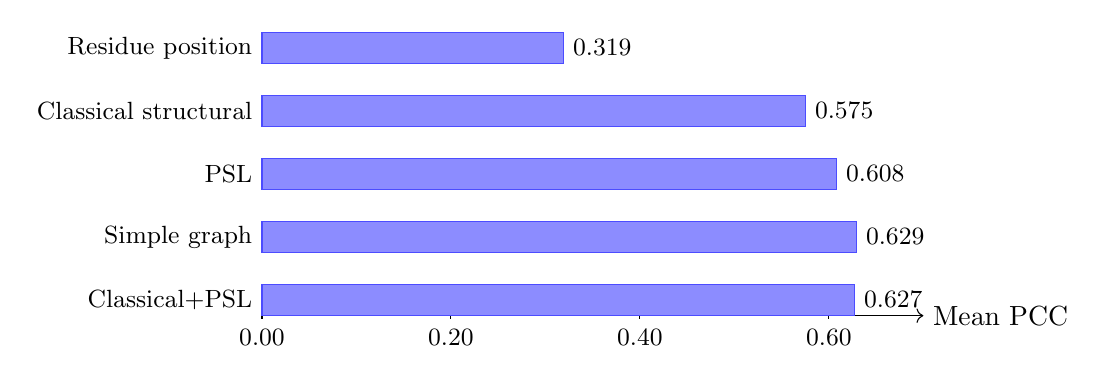
\begin{tikzpicture}[x=0.12cm,y=0.8cm]
\draw[->] (0,0) -- (70,0) node[right] {Mean PCC};
\foreach \x/\label in {0/0.00,20/0.20,40/0.40,60/0.60} {
  \draw (\x,0.06) -- (\x,-0.06) node[below] {\small \label};
}
\foreach \name/\val/\label/\y in {
  {Residue position}/31.9/0.319/4,
  {Classical structural}/57.5/0.575/3,
  {PSL}/60.8/0.608/2,
  {Simple graph}/62.9/0.629/1,
  {Classical+PSL}/62.7/0.627/0
} {
  \node[left] at (0,\y+0.25) {\small \name};
  \draw[fill=blue!45, draw=blue!70] (0,\y) rectangle (\val,\y+0.5);
  \node[right] at (\val,\y+0.25) {\small \label};
}
\end{tikzpicture}
\caption{Mean per-protein PCC for baseline feature sets.}
\label{fig:baseline_pcc}
\end{figure}

\subsection{SHAP Attributions Align with Flexible Residues}
The PSL+SHAP analysis gave mean predictive PCC of 0.595 across the full collection, close to the robust predictive benchmark. Absolute SHAP attribution strength showed moderate agreement with normalized B-factors: mean PCC 0.482 (95\% CI [0.465, 0.497]), mean Spearman correlation 0.311, and mean top-quintile Jaccard overlap 0.338 (95\% CI [0.326, 0.350]).

\begin{table}[htbp]
\centering
\caption{SHAP explanation-target agreement.}
\label{tab:shap_alignment}
\resizebox{\textwidth}{!}{%
\begin{tabular}{lrrrrr}
\toprule
Dataset & Proteins & Model PCC & SHAP PCC(abs) & SHAP PCC(signed) & Jaccard top20(abs) \\
\midrule
Small & 30 & 0.568 & 0.520 & 0.568 & 0.359 \\
Medium & 36 & 0.577 & 0.489 & 0.577 & 0.322 \\
Large & 34 & 0.563 & 0.438 & 0.563 & 0.330 \\
365-only & 264 & 0.605 & 0.482 & 0.605 & 0.339 \\
All & 364 & 0.595 & 0.482 & 0.595 & 0.338 \\
\bottomrule
\end{tabular}%
}
\end{table}

These results support an explanation-target association, not a causal interpretation of SHAP values. SHAP identifies which PSL features contribute most strongly to the model's predictions and where attribution strength concentrates relative to high-B-factor residues.

\subsection{Multiscale PSL Features at 9 and 12 Angstrom Dominate Attribution}
The highest mean absolute SHAP contributions came primarily from 9 and
12~\angstrom PSL features, especially \texttt{r9\_p0p0\_d0\_std},
\texttt{r12\_p0p0\_d0\_std}, \texttt{r9\_p0p0\_d0\_max}, and
\texttt{r12\_p0p0\_d0\_min}.

\begin{table}[htbp]
\centering
\caption{Top PSL feature attributions.}
\label{tab:shap_features}
\begin{tabular}{rlr}
\toprule
Rank & Feature & Mean absolute SHAP \\
\midrule
1 & \texttt{r9\_p0p0\_d0\_std} & 0.133 \\
2 & \texttt{r12\_p0p0\_d0\_std} & 0.106 \\
3 & \texttt{r9\_p0p0\_d0\_max} & 0.068 \\
4 & \texttt{r12\_p0p0\_d0\_min} & 0.056 \\
5 & \texttt{r6\_p0p0\_d0\_std} & 0.044 \\
6 & \texttt{r12\_p0p0\_d0\_mean} & 0.044 \\
\bottomrule
\end{tabular}
\end{table}

These features describe spectral properties of residue neighborhoods at intermediate-to-broad local scales. Their importance is consistent with the biophysical expectation that residue mobility is shaped by the surrounding packing environment and not solely by immediate nearest-neighbor geometry.

\begin{figure}[htbp]
\centering
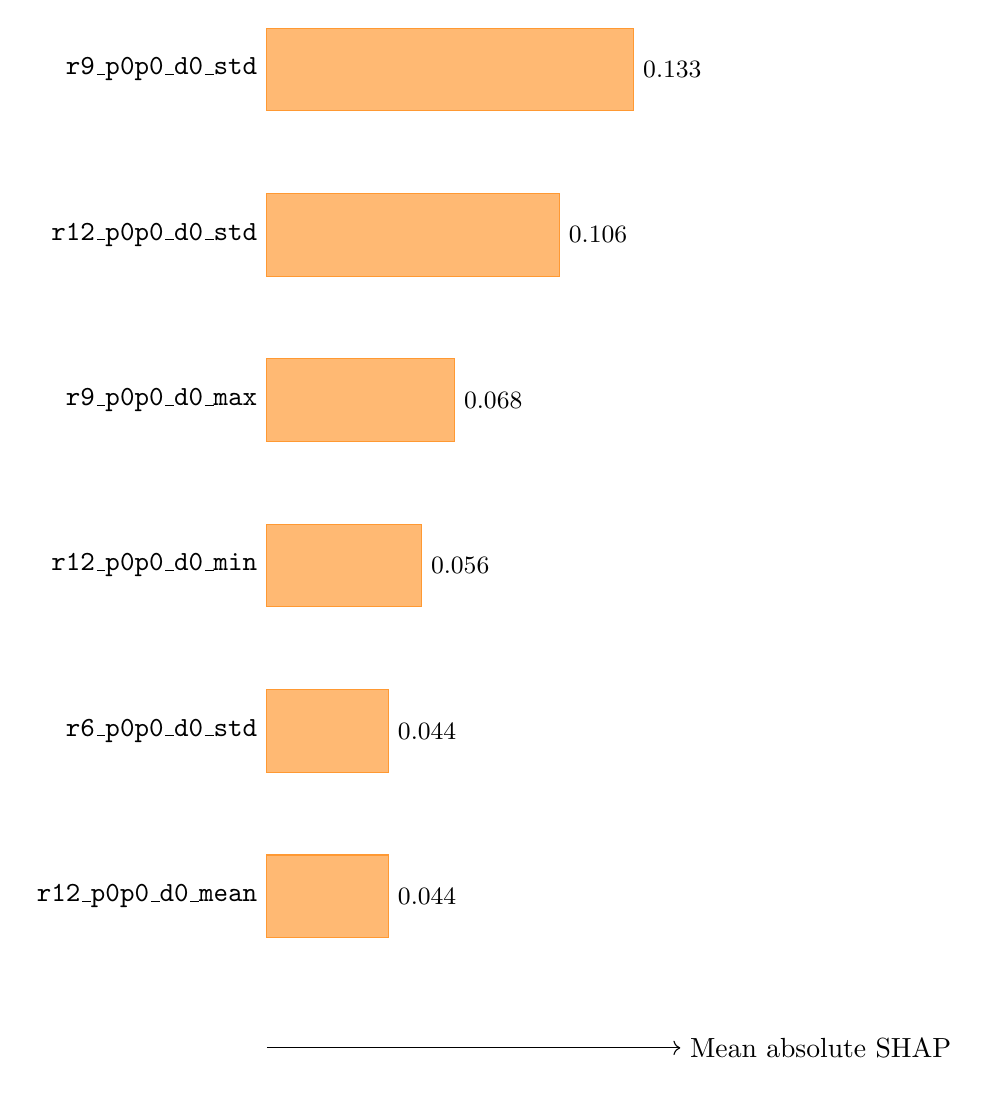
\begin{tikzpicture}[x=35cm,y=35cm]
\foreach \feature/\val/\label/\y in {
  {\texttt{r9\_p0p0\_d0\_std}}/0.133/0.133/0.42,
  {\texttt{r12\_p0p0\_d0\_std}}/0.106/0.106/0.36,
  {\texttt{r9\_p0p0\_d0\_max}}/0.068/0.068/0.30,
  {\texttt{r12\_p0p0\_d0\_min}}/0.056/0.056/0.24,
  {\texttt{r6\_p0p0\_d0\_std}}/0.044/0.044/0.18,
  {\texttt{r12\_p0p0\_d0\_mean}}/0.044/0.044/0.12
} {
  \node[left] at (0,\y+0.015) {\feature};
  \draw[fill=orange!55, draw=orange!80] (0,\y) rectangle (\val,\y+0.03);
  \node[right] at (\val,\y+0.015) {\small \label};
}
\draw[->] (0,0.08) -- (0.15,0.08) node[right] {Mean absolute SHAP};
\end{tikzpicture}
\caption{Dominant PSL attributions are concentrated at the 9 and 12~\angstrom neighborhood scales.}
\label{fig:shap_importance}
\end{figure}

\subsection{Biological Validation Confirms Expected Exposure, Packing, and Terminal Effects}
Independent structural annotations showed strong dataset-level agreement with known determinants of flexibility. Within-protein normalized B-factors were positively associated with solvent-accessible area and negatively associated with packing density. Flexible top-quintile residues were strongly enriched in solvent-exposed, under-packed, and terminal positions.

\begin{table}[htbp]
\centering
\caption{Biological validation of normalized B-factor labels.}
\label{tab:biological_validation}
\begin{tabular}{lrrr}
\toprule
Metric & Estimate & 95\% CI & Bootstrap $p$ \\
\midrule
Spearman($\zB$, solvent-accessible area) & 0.433 & [0.416, 0.449] & $<0.001$ \\
Spearman($\zB$, packing density 1) & -0.076 & [-0.090, -0.063] & $<0.001$ \\
Spearman($\zB$, packing density 2) & -0.400 & [-0.414, -0.385] & $<0.001$ \\
Spearman($\zB$, packing density 3) & -0.411 & [-0.426, -0.396] & $<0.001$ \\
AUC(flexible top20 from solvent area) & 0.730 & [0.721, 0.740] & $<0.001$ \\
AUC(flexible top20 from low packing density 3) & 0.743 & [0.734, 0.753] & $<0.001$ \\
Odds ratio: flexible if area top quartile & 4.663 & [4.227, 5.195] & $<0.001$ \\
Odds ratio: flexible if packing3 bottom quartile & 6.202 & [5.586, 6.887] & $<0.001$ \\
Odds ratio: flexible if terminal decile & 4.672 & [3.071, 6.742] & $<0.001$ \\
\bottomrule
\end{tabular}
\end{table}

The magnitude and direction of these associations are biologically coherent: surface-exposed residues have fewer stabilizing contacts, under-packed residues experience weaker local constraints, and terminal residues are often less restricted than internal residues.

\subsection{Secondary-Structure Patterns Are Consistent with Exposure and Packing}
Secondary-structure codes showed distinct normalized B-factor distributions. Codes 5 and 6 had the largest mean normalized B-factors and the highest fractions of flexible top-quintile residues, while code 4 had the lowest mean normalized B-factor and the smallest flexible fraction among common classes.

\begin{table}[htbp]
\centering
\caption{Secondary-structure-code summary.}
\label{tab:secondary_structure}
\begin{tabular}{rrrrr}
\toprule
sec\_type & Residues & Mean $\zB$ & Flexible top20 fraction & Mean area \\
\midrule
1 & 808 & -0.192 & 0.137 & 34.091 \\
2 & 3,060 & 0.153 & 0.257 & 60.422 \\
3 & 23,425 & -0.124 & 0.158 & 47.899 \\
4 & 19,658 & -0.396 & 0.082 & 30.545 \\
5 & 13,434 & 0.389 & 0.314 & 62.459 \\
6 & 14,825 & 0.347 & 0.322 & 62.710 \\
\bottomrule
\end{tabular}
\end{table}

These patterns reinforce the annotation-level validation: high-flexibility classes also tend to be more solvent exposed and less densely packed.

\FloatBarrier

\section{Discussion}
This study shows that PSL descriptors provide a reproducible, biologically interpretable signal for residue-level protein flexibility under protein-grouped evaluation. The observed predictive performance is moderate rather than exhaustive, which is scientifically plausible for a target as heterogeneous as crystallographic B-factor. B-factors combine true mobility, static disorder, model refinement, crystal contacts, occupancy, and experimental resolution; a structure-only model should not be expected to explain all of that variance.

The descriptor sensitivity experiments also temper the interpretation. Center labeling changed the spectra and improved the variability of zero-eigenvalue features, but it did not produce a large predictive jump. The 18-feature center-labeled descriptor was only modestly stronger than the 15-feature center-labeled variants, and increasing the Random Forest from 1,000 to 2,000 trees gave essentially unchanged performance. This supports treating the measured PSL signal as a stable estimate for this descriptor family rather than as an artifact of tree count alone.

The protocol-comparability analyses clarify the relationship between these results and specific PSL flexibility experiments reported by Hayes et al. The PSL-only linear approximation corresponding to their Table~1 reached mean PCC 0.707 only when the linear model was fit separately within each protein; pooled OLS was substantially lower by per-protein PCC. Protein-level raw-B-factor models following their blind-prediction setup reached mean per-protein PCCs near 0.60. Under random residue-level splitting, annotation+PSL features reached pooled PCCs above 0.85, but their mean per-protein PCCs remained near 0.61--0.64. Classical structural and simple graph controls showed the same pooled-metric jump under random residue splits. This pattern indicates that high apparent accuracy is reproducible under atom-level comparability protocols, while protein-level evaluation gives a more moderate estimate of how much residue-flexibility signal transfers across structures.

The explanation analysis supports a coherent mechanistic reading. The most important PSL features arise at 9 and 12~\angstrom radii, scales large enough to capture local packing and neighborhood organization beyond immediate bonded contacts. The biological validation independently confirms that high normalized B-factors are enriched among exposed, under-packed, and terminal residues. Thus, the PSL model is not merely detecting arbitrary numerical patterns in the target array; it is using geometric descriptors that align with known physical determinants of residue mobility.

The results also illustrate a useful standard for explainable machine learning in structural biology: explanation metrics should be reported alongside predictive metrics and interpreted as model diagnostics. Here, SHAP attribution alignment is moderate, reinforcing the view that PSL features carry meaningful geometric signal without implying causal identification of flexibility determinants.

The baseline comparisons sharpen the representation claim. PSL descriptors outperform the classical structural baseline, indicating that PSL spectra capture geometric information beyond the supplied exposure, packing, secondary-structure, and position annotations. However, the simple \calpha graph baseline is also strong, and the combined classical+PSL model is close to but does not exceed the graph baseline by mean per-protein PCC. The most defensible interpretation is therefore that PSL features contribute useful multiscale geometric signal, but their value is complementary rather than exclusive.

\section{Limitations}
B-factors are imperfect proxies for dynamics. They are influenced by refinement choices, crystal contacts, temperature, occupancy, and structure quality. Within-protein normalization reduces some scale variation but does not isolate true conformational mobility from all crystallographic effects.

The SHAP analysis used a 25-tree interpretability model for computational tractability. Its predictive PCC closely matched the larger robust forest, but future work should report runtime-optimized full-model explanations or compare multiple explanation backends.

The secondary-structure table is reported by numeric source codes because the annotation files do not include a codebook. A future structural annotation pass with DSSP would allow named class-level conclusions.

The model is evaluated on B-factor labels from a single dataset family. External benchmarking against independent crystallographic collections, NMR-derived order parameters, hydrogen-deuterium exchange, or molecular dynamics ensembles would further test the biological scope of the learned signal. Homology and structural redundancy should also be quantified before strong claims are made about generalization to remote protein families.

The blind-prediction reproduction runs based on Hayes et al.'s setup used B-factor subsequence alignment when annotation tables and \calpha PSL rows differed in length. This retained 56 proteins that would otherwise be dropped, but 17 proteins still failed row alignment. A residue-identifier mapping using chain ID, residue number, and insertion code would be preferable for exact reproduction of annotation-rich blind-prediction datasets.

Finally, SHAP is a model-dependent attribution method, not a causal analysis. The reported SHAP metrics indicate agreement between model attributions and B-factor patterns; they do not prove that specific PSL eigenvalue statistics are causal determinants of flexibility.

\section{Conclusion}
Center-labeled persistent sheaf Laplacian features encode multiscale local geometry that supports prediction of normalized residue B-factors. SHAP analysis links model attributions to flexible residues, and independent annotation tests show that the target labels follow established biological determinants of mobility: solvent exposure, weak packing, and terminal position. Protocol-comparability analyses further show that high raw-B-factor accuracy is attainable under atom-level splitting, whereas protein-level evaluation supports a more moderate generalization claim. Together, these results establish a rigorous and reproducible framework for explainable PSL-based protein-flexibility modeling.

\section*{Data and Code Availability}
The analysis code is organized as command-line scripts with a minimal Python package namespace. The public repository is available at:
\begin{center}
\small\url{https://github.com/ryan-charette/psl-protein-flexibility}
\end{center}
Third-party structures and annotation tables are expected from the MDG\_bfactor dataset and are not tracked in the repository. Lightweight metric snapshots are provided under \texttt{results/metrics/}; full predictions and generated PSL matrices can be regenerated from the documented commands. The repository also documents how to supply the upstream PSL implementation locally, because that third-party source file is not redistributed in the public package.

\begin{thebibliography}{99}

\bibitem[Atilgan et~al.(2001)]{atilgan2001}
Atilgan, A.~R., Durell, S.~R., Jernigan, R.~L., Demirel, M.~C.,
Keskin, O., and Bahar, I. (2001).
Anisotropy of fluctuation dynamics of proteins with an elastic network model.
\textit{Biophysical Journal}, 80(1), 505--515.

\bibitem[Bahar et~al.(2010)]{bahar2010}
Bahar, I., Lezon, T.~R., Yang, L.-W., and Eyal, E. (2010).
Global dynamics of proteins: bridging between structure and function.
\textit{Annual Review of Biophysics}, 39, 23--42.

\bibitem[Edelsbrunner and Harer(2010)]{edelsbrunner2010}
Edelsbrunner, H. and Harer, J. (2010).
\textit{Computational Topology: An Introduction}.
American Mathematical Society.

\bibitem[Feng et~al.(2025)]{feng2025}
Feng, H., Zhao, J.~Y., and Wei, G.-W. (2025).
Multiscale differential geometry learning for protein flexibility analysis.
\textit{Journal of Computational Chemistry}, 46, e70073.
doi:10.1002/jcc.70073.

\bibitem[Hayes et~al.(2025a)]{hayes2025}
Hayes, N., Wei, X., Feng, H., Merkurjev, E., and Wei, G.-W. (2025).
Persistent sheaf Laplacian analysis of protein flexibility.
\textit{Journal of Physical Chemistry B}, 129(17), 4169--4178.
doi:10.1021/acs.jpcb.5c01287.

\bibitem[Hayes et~al.(2025b)]{hayes2025correction}
Hayes, N., Wei, X., Feng, H., Merkurjev, E., and Wei, G.-W. (2025).
Correction to ``Persistent sheaf Laplacian analysis of protein flexibility.''
\textit{Journal of Physical Chemistry B}, 129(24), 6112--6113.
doi:10.1021/acs.jpcb.5c03679.

\bibitem[Haliloglu et~al.(1997)]{haliloglu1997}
Haliloglu, T., Bahar, I., and Erman, B. (1997).
Gaussian dynamics of folded proteins.
\textit{Physical Review Letters}, 79(16), 3090--3093.

\bibitem[Lundberg and Lee(2017)]{lundberg2017}
Lundberg, S.~M. and Lee, S.-I. (2017).
A unified approach to interpreting model predictions.
\textit{Advances in Neural Information Processing Systems}, 30.

\bibitem[Nguyen et~al.(2016)]{nguyen2016}
Nguyen, D.~D., Xia, K., and Wei, G.-W. (2016).
Generalized flexibility-rigidity index.
\textit{Journal of Chemical Physics}, 144(23), 234106.

\bibitem[Xia and Wei(2014)]{xia2014}
Xia, K. and Wei, G.-W. (2014).
Persistent homology analysis of protein structure, flexibility, and folding.
\textit{International Journal for Numerical Methods in Biomedical Engineering},
30(8), 814--844.

\end{thebibliography}

\end{document}
